\documentclass[11pt]{article}

% ---------- Packages ----------
\usepackage[margin=1in]{geometry}
\usepackage{amsmath,amsthm,graphicx,enumitem,amssymb}
\usepackage{mathtools}
\usepackage{physics}        % derivatives, bras/kets, etc.
\usepackage{siunitx}        % units
\usepackage{graphicx}       % figures
\usepackage{float}          % figure placement
\usepackage{booktabs}       % nice tables
\usepackage{enumitem}       % better lists
\usepackage{fancyhdr}       % header/footer
\usepackage{titlesec}       % section formatting
\usepackage{hyperref}       % links
\usepackage{tcolorbox}      % boxes for answers
\usepackage{listings}       % code (MATLAB, Python, etc.)
\usepackage{xcolor}
\usepackage{bbm}        % blackboard bold italic
\usepackage{tikz}
\usetikzlibrary{automata, positioning, arrows.meta, bending, decorations.pathmorphing}
\usepackage{etoolbox}
\usepackage{bbm}


% ---------- Hyperref Setup ----------
\hypersetup{
    colorlinks=true,
    linkcolor=blue,
    urlcolor=blue,
    citecolor=blue
}

% ---------- Header/Footer ----------
\pagestyle{fancy}
\fancyhf{}
\lhead{\textbf{\course}}
\rhead{\textbf{\assignment}}
\cfoot{\thepage}

% ---------- Custom Commands ----------
\newcommand{\course}{ASEN 5264 -- DMU}
\newcommand{\assignment}{Homework \#3}
\newcommand{\studentname}{Bijan Jourabchi}
\newcommand{\studentid}{Student ID}

\newcommand{\R}{\mathbb{R}}
\newcommand{\E}{\mathbb{E}}
\newcommand{\Var}{\mathrm{Var}}
\newcommand{\Cov}{\mathrm{Cov}}

% Boxed answer environment
\newtcolorbox{answerbox}{
    colback=gray!5,
    colframe=gray!50,
    title=Answer,
    fonttitle=\bfseries
}

% Problem section format
\titleformat{\section}{\large\bfseries}{Problem \thesection:}{0.5em}{}

% ---------- Code Style ----------
\lstset{
    basicstyle=\ttfamily\small,
    keywordstyle=\color{blue},
    commentstyle=\color{green!50!black},
    stringstyle=\color{orange},
    breaklines=true,
    frame=single
}

% ---------- Document ----------
\begin{document}

% ---------- Title Block ----------
\begin{center}
    {\LARGE \textbf{\course}} \\[6pt]
    {\Large \assignment} \\[10pt]
    \studentname \\
    ID: \studentid \\
\end{center}

\vspace{1em}
\hrule
\vspace{1em}

% =====================================================
\section{}

\begin{enumerate}[label=\alph*)]
    % =====================================================
    \item
    Given $U^*$ we can extract the optimal policy $\pi^*$ from $U^*$ with the following expression:
    \[
        \pi^*(s) = \arg\max_{a \in A}(R(s,a) + \gamma \mathbb{E}[U^*(s)])
    \]
    % =====================================================
    \item
    We are given an MDP defined by, \newline
    $S = \mathbb{R},  \quad A = \{0,0.1,1\}, \quad \gamma = 1$ \newline
    $T(s' \mid s,a) = \mathcal{U}([s+a,s+a+1])$ \newline
    $R(s,a) = -\mathbbm{1}(s \leq 1) - a$ \newline
    $U^{\tilde{\pi}}(s) = -2\cdot\mathbbm{1}(s \leq 1)$

    Where $\mathcal{U}([s+a,s+a+1])$ represents a uniform distribution from $s+a$ to $s+a+1$, and $\mathbbm{1}(s \leq 1)
    = 1$ if $s \leq 1$ and $0$ otherwise. Given $s = 0.8$, we must find the action which maximizes $Q^{\tilde{\pi}}(s,a)$,
    which is given by
    \[
        Q^{\tilde{\pi}}(s,a) = R(s,a) + \sum_{s'} T(s' \mid s,a)U^{\tilde{\pi}}(s')
    \]

    Since there are only three actions, we can compute $Q^{\tilde{\pi}}(s=0.8,a)$ for $\forall a \in A$. Since, $S$ and $T$ are continous,
    we also note that the summation will be an integral over all of the possible future state $s'$. Thus, our expression for $Q^{\tilde{\pi}}(s,a)$
    becomes 
    \[
        Q^{\tilde{\pi}}(0.8,a) = R(0.8,a) + \int_{-\infty}^{\infty} T(s' \mid 0.8,a)U^{\tilde{\pi}}(s') ds'
    \]

    We can now compute $Q^{\tilde{\pi}}(0.8,a)$ for all a $\in$ A, begining with $a = 0$. Note that $\mathcal{U}([s+a,s+a+1]) = 1 \ \forall \ a,s$ by definition
    of the uniform distribution. \newline

    a = 0:

    \[
    \begin{aligned}
        Q^{\tilde{\pi}}(0.8,0) &= R(0.8,0) + \int_{-\infty}^{\infty} T(s' \mid 0.8,0)U^{\tilde{\pi}}(s') ds' \\ 
        Q^{\tilde{\pi}}(0.8,0) &= (-\mathbbm{1}(0.8 \leq 1) - 0) + \int_{-\infty}^{\infty} \mathcal{U}([0.8,1.8])(-2\cdot\mathbbm{1}(s' \leq 1)) ds' \\
        Q^{\tilde{\pi}}(0.8,0) &= -1 + \int_{-\infty}^{\infty} (-2\cdot\mathbbm{1}(s' \leq 1)) ds' \\
        Q^{\tilde{\pi}}(0.8,0) &= - 1 + \int_{0.8}^1 -2 ds' = -1 - 2(0.2) = -1.4
    \end{aligned}
    \]

    a = 0.1:

    \[
    \begin{aligned}
        Q^{\tilde{\pi}}(0.8,0.1) &= R(0.8,0.1) + \int_{-\infty}^{\infty} T(s' \mid 0.8,0.1)U^{\tilde{\pi}}(s') ds' \\ 
        Q^{\tilde{\pi}}(0.8,0.1) &= (-\mathbbm{1}(0.8 \leq 1) - 0.1) + \int_{-\infty}^{\infty} (-2\cdot\mathbbm{1}(s' \leq 1)) ds' \\
        Q^{\tilde{\pi}}(0.8,0.1) &= -1.1 + \int_{0.9}^{1.9} (-2\cdot\mathbbm{1}(s' \leq 1)) ds' \\
        Q^{\tilde{\pi}}(0.8,0.1) &= - -1.1 + \int{0.9}^{1} -2 ds' = -1.1 - 2(0.1) = -1.3 
    \end{aligned}
    \]

    a = 1:

    \[
    \begin{aligned}
        Q^{\tilde{\pi}}(0.8,1) &= R(0.8,1) + \int_{-\infty}^{\infty} T(s' \mid 0.8,1)U^{\tilde{\pi}}(s') ds' \\ 
        Q^{\tilde{\pi}}(0.8,1) &= (-\mathbbm{1}(0.8 \leq 1) - 1) + \int_{-\infty}^{\infty} (-2\cdot\mathbbm{1}(s' \leq 1)) ds' \\
        Q^{\tilde{\pi}}(0.8,1) &= -2 + \int_{1.8}^{2.8} (-2\cdot\mathbbm{1}(s' \leq 1)) ds' \\
        Q^{\tilde{\pi}}(0.8,1) &= -2
    \end{aligned}
    \]

    Thus. the action which minimizes $Q^{\tilde{\pi}}(0.8,a)$ is \boxed{$a = 0.1$}.

\end{enumerate}



% =====================================================
\section{}

Given the following MDP:


    \begin{figure}[H]
        \centering
        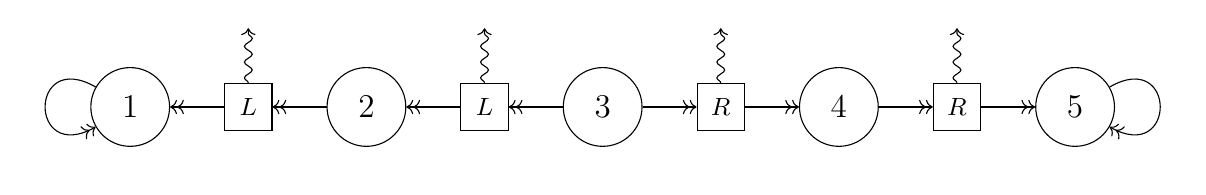
\begin{tikzpicture}[
            state/.style = {circle, draw, minimum size=1.0cm, font=\large},
            action/.style = {rectangle, draw, minimum size=0.6cm, font=\small},
            every edge/.style = {draw, thick},
        ]
            % States in a horizontal line
            \node[state] (1) at (0,0) {$1$};
            \node[state] (2) at (3,0) {$2$};
            \node[state] (3) at (6,0) {$3$};
            \node[state] (4) at (9,0) {$4$};
            \node[state] (5) at (12,0) {$5$};

            % Action nodes between states
            \node[action] (L1) at (1.5,0) {$L$};
            % \node[] (R1) at (1.5,1.25) {$1$};
            \node[action] (L2) at (4.5,0) {$L$};
            \node[action] (R3) at (7.5,0) {$R$};
            \node[action] (R4) at (10.5,0) {$R$};

            % Transitions: arrows point away from state 3
            % 3 -> L -> 2 -> L -> 1 (left side)
            \draw[->>] (3) -- (L2);
            \draw[->>] (L2) -- (2);
            \draw[->>] (2) -- (L1);
            \draw[->>] (L1) -- (1);
            % 3 -> R -> 4 -> R -> 5 (right side)
            \draw[->>] (3) -- (R3);
            \draw[->>] (R3) -- (4);
            \draw[->>] (4) -- (R4);
            \draw[->>] (R4) -- (5);

            % Absorbing state loops
            \draw[->>] (1) to[out=150, in=210, looseness=5] (1);
            \draw[->>] (5) to[out=30, in=-30, looseness=5] (5);

            % Reward arrows (squiggly) from action nodes
            \draw[->, decorate, decoration={snake, amplitude=0.5mm, segment length=2mm}] (L1) -- ++(0,1); 
            \draw[->, decorate, decoration={snake, amplitude=0.5mm, segment length=2mm}] (L2) -- ++(0,1);
            \draw[->, decorate, decoration={snake, amplitude=0.5mm, segment length=2mm}] (R3) -- ++(0,1);
            \draw[->, decorate, decoration={snake, amplitude=0.5mm, segment length=2mm}] (R4) -- ++(0,1);
        \end{tikzpicture}
    \end{figure}

    We are asked to disprove the following statement:     
    \begin{quote}
    If a policy $\pi$ satisfies $|Q^*(s, \pi^*(s)) - Q^*(s, \pi(s))| \leq \beta$ for all $s \in S$ for some $\beta > 0$, then it immediately follows that $|R(s, \pi^*(s)) - R(s, \pi(s))| \leq \beta$ for any $s \in S$.
    \end{quote}
    In order to find a counter example, we must find a reward function, $R$ a policy $\pi$, and a value $\beta$ that disproves the claim. Since all transitions are deterministic, and 
    every state other than $s = 3$ only has a single action we only have to choose $\pi(3)$ and $\pi^*(3)$, the optimal policy. When choosing $R(s,a)$, we will ensure that one action at $s = 3$ is clearly better than the other action,
    that way our policy will differ from the optimal policy which is necessary to disprove the statement. To disprove the claim, consider the following reward function for our MDP:

        \begin{figure}[H]
        \centering
        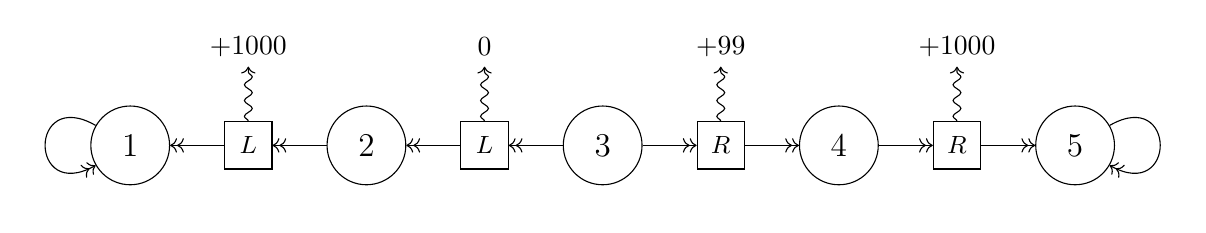
\begin{tikzpicture}[
            state/.style = {circle, draw, minimum size=1.0cm, font=\large},
            action/.style = {rectangle, draw, minimum size=0.6cm, font=\small},
            every edge/.style = {draw, thick},
        ]
            % States in a horizontal line
            \node[state] (1) at (0,0) {$1$};
            \node[state] (2) at (3,0) {$2$};
            \node[state] (3) at (6,0) {$3$};
            \node[state] (4) at (9,0) {$4$};
            \node[state] (5) at (12,0) {$5$};

            % Action nodes between states
            \node[action] (L1) at (1.5,0) {$L$};
            \node[] (R1) at (1.5,1.25) {$+1000$};
            \node[action] (L2) at (4.5,0) {$L$};
            \node[] (R1) at (4.5,1.25) {$0$};
            \node[action] (R3) at (7.5,0) {$R$};
            \node[] (R1) at (7.5,1.25) {$+99$};
            \node[action] (R4) at (10.5,0) {$R$};
            \node[] (R1) at (10.5,1.25) {$+1000$};

            % Transitions: arrows point away from state 3
            % 3 -> L -> 2 -> L -> 1 (left side)
            \draw[->>] (3) -- (L2);
            \draw[->>] (L2) -- (2);
            \draw[->>] (2) -- (L1);
            \draw[->>] (L1) -- (1);
            % 3 -> R -> 4 -> R -> 5 (right side)
            \draw[->>] (3) -- (R3);
            \draw[->>] (R3) -- (4);
            \draw[->>] (4) -- (R4);
            \draw[->>] (R4) -- (5);

            % Absorbing state loops
            \draw[->>] (1) to[out=150, in=210, looseness=5] (1);
            \draw[->>] (5) to[out=30, in=-30, looseness=5] (5);

            % Reward arrows (squiggly) from action nodes
            \draw[->, decorate, decoration={snake, amplitude=0.5mm, segment length=2mm}] (L1) -- ++(0,1); 
            \draw[->, decorate, decoration={snake, amplitude=0.5mm, segment length=2mm}] (L2) -- ++(0,1);
            \draw[->, decorate, decoration={snake, amplitude=0.5mm, segment length=2mm}] (R3) -- ++(0,1);
            \draw[->, decorate, decoration={snake, amplitude=0.5mm, segment length=2mm}] (R4) -- ++(0,1);
        \end{tikzpicture}
    \end{figure}

    It is clear that the optimal policy at $s = 3$ is $\pi^*(3) = R$, so we will choose our policy to be $\pi(3) = L$. Next, we will use the Bellman Backup
    algorithm in order to compute values for $Q(s,\pi)$. Since we have two terminal states, $s = 1$ and $s = 5$, we will start there and work back until we can compute
    $Q(3,\pi) = R(3,\pi(3)) + 0.9 U^{\pi}(s')$ for both the optimal policy and non-optimal policy, \newline \newline

    \begin{tabular}{|l|l|l|l|}
    \hline
    S & A    & $Q^*$ & $V^*$ \\ \hline
    1 & N/A  & 0                  & 0                    \\ \hline
    5 & N/A  & 0                  & 0                    \\ \hline
    4 & R & 1000 & 1000 \\ \hline
    2 & L & 1000 & 1000 \\ \hline
    3 & R & 99 + 0.9(1000) = 999 & 999 \\ \hline
    3 & L & 0.9(1000) = 900 &  \\ \hline
    \end{tabular} \newline \newline

    Thus, we get $Q(3,\pi^*(3)) = 999$ and $Q(3,\pi(3)) = 900$. Finally, let's select $\beta = 99.5$.
    Our policy satisfies $|Q^*(3, \pi^*(3)) - Q^*(3, \pi(3))| \leq \beta \rightarrow |999 - 900| \leq 99.5 \rightarrow 99 \leq 99.5$. 
    The original claim states that it immediately follows that $|R(3, \pi^*(3)) - R(3, \pi(3))| \leq \beta$. However, we see that 
    $|100 - 0| = 100 \nleq 99.5$. Thus, we have found a counter example for the claim.

% =====================================================

\end{document}